% This is "sig-alternate.tex" V2.0 May 2012
% This file should be compiled with V2.5 of "sig-alternate.cls" May 2012
%
% For tracking purposes - this is V2.0 - May 2012

\documentclass[prodmode,acmtap]{acmlarge}

\usepackage{graphicx}
\usepackage{subfigure}
\usepackage{url}
\usepackage{times}
%\usepackage{cite}
%\usepackage[T1]{fontenc}
\usepackage{color}
\newcommand{\red}[1]{\textcolor{red}{#1}}
\newcommand{\blue}[1]{\textcolor{blue}{#1}}

%\usepackage[normalem]{ulem}


\begin{document}

\title{To What Extent ACM SIG Conferences Communities are Connected?}

\author{Fabr��cio Benevenuto, Alberto H. F. Laender, Bruno Leite Alves \\
\affil{Universidade Federal de Minas Gerais, Brazil}
}


%\category{H.2.8}{Database Management}{Database Applications}[Data Mining]
%\terms{Measurement}
%\keywords{h-index}





\maketitle
\begin{abstract}

\noindent
There have been considerable efforts in the literature towards understanding and modeling dynamic aspects of 
scientific communities. Despite the great interest, little is known about the role that different members play 
in the formation of the underlying network structure of such communities. In this paper, we provide a wide 
investigation of the roles that members of the core of scientific communities play in the collaboration network 
structure formation and evolution. To do that, we define a community core based on an individual metric, 
\textit{core score}, which is an h-index derived metric that captures both, the prolificness and the involvement
of researchers in a community. Our results provide a number of key observations related to community formation and 
evolving patterns. Particularly, we show that members of the community core work as bridges that connect smaller 
clustered research groups. Furthermore, these members are responsible for an increase in 
the average degree of the whole community underlying network and a decrease on the overall network assortativeness. 
More important, we note that variations on the members of the community core tend to be strongly correlated with 
variations on these metrics. We argue that our observations are important for shedding a light on the role of key 
members on community formation and structure.
\end{abstract}

\category{J.4.} {Computer Applications} Social and Behavioral Sciences
\terms{Human Factors, Measurement.}
\keywords{Scientific Communities, Core Community, Community Evolution.}
\vspace{1.4cm}


\section{Introduction}


\red{1 - Write about the creation of the SIG conferences and their role to connect authors. \\
2 - The thing has evolved and there are several SIGs. \\
3 - To what extend SIGs are able to connect the important researchers of an specific research area? \\
4 - We developed the follwoing methodology to investigate this question. \\
5 - Our results show that most of the SIGs are able to connect their main authors in connected components. Only a few SIGs, with specific characteristics do not achieve this
property.`
}




\section{Scientific Communities}

\red{Goal here is to visualize communities, but not only the coauthorship network of all authors. We want two things: 
1 - Investigate connectivity among authors of specific SIG communities. \\
2 - We want to be able to identify the most prolific researchers with high level of participation in a community. }


The notion of community can be understood as a dense group of nodes in a network, with more edges inside than edges linking the rest of the network.  There are multiple definitions
and strategies for identifying communities and they vary according to the context~\cite{Kleinberg@cacm2008,Leskovec@www2010}. In our context, a scientific community is defined in terms of a large and well established
scientific conference able to aggregate researchers working in similar research topics along a considerable number of years. 


In order to construct a set of scientific communities, we have gathered data from DBLP\footnote{http://dblp.uni-trier.de/}~\cite{Ley:2009}, a digital library containing more
than 2.2 million publications from 1.2 million authors that provides bibliographic information on major Computer Science conference proceedings and journals.  DBLP offers its
entire database in XML format, which facilitates gathering and constructing entire scientific communities. 

Each publication is accompanied by its title, list of authors, year of publication, and publication venue, i.e., a conference or journal. For the purposes of our work, we
consider a scientific community as a graph in which nodes represent researchers and edges links coauthors of papers from the same community.  In order to define such communities,
we focus on the publications from the flagship conferences of major ACM SIGs (Special Interest Groups).  Thus, we define a scientific community by linking people that have
coauthored a paper in a certain conference, making the flagship conferences of the ACM SIGs to act as communities where coauthorships are formed. We have removed young conferences
without enough data for a temporal analysis as well as conferences whose entire history is not registered on DBLP to allow us carrying out temporal analyses. 

In total, 24 scientific communities were constructed. Table~\ref{tab:sigs_conference_period} lists these communities, including the respective ACM SIG, the conference acronym, the period
considered (some conferences had the period reduced to avoid hiatus in the data), the total number of authors, publications and editions as well as ratios extracted from these last three figures.

\begin{table}[!htb]
\centering
\caption{DBLP statistics on the flagship conferences of ACM SIGs}
\label{tab:sigs_conference_period}
\begin{tabular}{|l|l|c|c|c|c|c|c|c|c|} \hline
\bf{SIG} & \bf{Conference} & \bf{Period} & \bf{Authors} & \bf{Publications} & \bf{Editions} & \bf{Aut/Edi} & \bf{Pub/Edi} & \bf{Aut/Pub}\\ \hline
SIGACT & STOC & 1969-2012 & 2159 & 2685 & 44 & 49.07 & 61.02 & 0.80\\ \hline
SIGAPP & SAC & 1993-2011 & 9146 & 4500 & 19 & 481.37 & 236.84 & 2.03\\ \hline
SIGARCH & ISCA & 1976-2011 & 2461 & 1352 & 36 & 68.36 & 37.56 & 1.82\\ \hline
SIGBED & HSCC & 1998-2012 & 846 & 617 & 15 & 56.40 & 41.13 & 1.37\\ \hline
SIGCHI & CHI & 1994-2012 & 5095 & 2819 & 19 & 268.16 & 148.37 & 1.81\\ \hline
SIGCOMM & SIGCOMM & 1988-2011 & 1593 & 796 & 24 & 66.38 & 33.17 & 2.00\\ \hline
SIGCSE & SIGCSE & 1986-2012 & 3923 & 2801 & 27 & 145.30 & 103.74 & 1.40\\ \hline
SIGDA & DAC & 1964-2011 & 8876 & 5693 & 48 & 184.92 & 118.60 & 1.56\\ \hline
SIGDOC & SIGDOC & 1989-2010 & 1071 & 810 & 22 & 48.68 & 36.82 & 1.32\\ \hline
SIGGRAPH & SIGGRAPH & 1985-2003 & 1920 & 1108 & 19 & 101.05 & 58.32 & 1.73\\ \hline
SIGIR & SIGIR & 1978-2011 & 3624 & 2687 & 34 & 106.59 & 79.03 & 1.35\\ \hline
SIGKDD & KDD & 1995-2011 & 3078 & 1699 & 17 & 181.06 & 99.94 & 1.81\\ \hline
SIGMETRICS & SIGMETRICS & 1981-2011 & 2083 & 1174 & 31 & 67.19 & 37.87 & 1.77\\ \hline
SIGMICRO & MICRO & 1987-2011 & 1557 & 855 & 25 & 62.28 & 34.20 & 1.82\\ \hline
SIGMM & MM & 1993-2011 & 5400 & 2928 & 19 & 284.21 & 154.11 & 1.84\\ \hline
SIGMOBILE & MOBICOM & 1995-2011 & 1151 & 480 & 17 & 67.71 & 28.24 & 2.40\\ \hline
SIGMOD & SIGMOD & 1975-2012 & 4202 & 2669 & 38 & 110.58 & 70.24 & 1.57\\ \hline
SIGOPS & PODC & 1982-2011 & 1685 & 1403 & 30 & 56.17 & 46.77 & 1.20\\ \hline
SIGPLAN & POPL & 1975-2012 & 1527 & 1217 & 38 & 40.18 & 32.03 & 1.25\\ \hline
SIGSAC & CCS & 1996-2011 & 1354 & 676 & 16 & 84.63 & 42.25 & 2.00\\ \hline
SIGSAM & ISSAC & 1988-2011 & 1100 & 1177 & 24 & 45.83 & 49.04 & 0.93\\ \hline
SIGSOFT & ICSE & 1987-2011 & 3502 & 2248 & 25 & 140.08 & 89.92 & 1.56\\ \hline
SIGUCCS & SIGUCCS & 1989-2011 & 1771 & 1593 & 23 & 77.00 & 69.26 & 1.11\\ \hline
SIGWEB & CIKM & 1992-2011 & 4978 & 2623 & 20 & 248.90 & 131.15 & 1.90\\ \hline
\end{tabular}
\end{table}



\section{Defining a Community Core}

Previous attempts for identifying the community core of a scientific community are based on algorithmic approaches that aim at identifying dense clusters of nodes in the
network~\cite{Seifi:2012:CCE:2187980.2188258}.  However, as we plan to investigate the role of a core in the network structure, any approach that makes use of the network structure
to identify such nodes could lead us to a biased set of researchers. Instead, we focus on developing a metric that quantifies the involvement of a researcher in a scientific community
during a certain period of time.  Intuitively, this metric should be able to capture (i) the prolificness of a researcher in different communities and (ii) the frequency of involvement
of that researcher with the community in a certain period of time.

First, in order to capture the prolificness of a researcher, we use the h-index~\cite{Hirsch:2005}, a metric widely adopted for this purpose. This metric consists of an index that
attempts to measure both the productivity and the impact of the published work of a researcher. It is based on the set of the researcher's most cited papers and the number of
citations that they have received.  More specifically, a researcher $r$ has an h-index $h_r$ if she has published \textit{h} papers which have received at least \textit{h} citations. Thus, for
example, if a researcher has 10 papers with at least 10 citations, her h-index is 10.  

Second, as an attempt to capture the importance of a researcher to a specific community in a certain period of time, we multiple her h-index by the number of publications this
researcher has in a certain community during a time window. We name this metric \textit{Core Score}. More formally, the Core Score of a researcher $r$ in a community $c$ during a period of
time $t$, $Core{ }Score_{r,c,t}$, is given by its h-index $h_r$ multiplied by the number of publications $r$ has in $c$ during $t$ ($\textrm{\#}publications_{r,c,t}$),
as expressed by Equation~\ref{eq:core_score}. 
\vspace{-0.01cm}
\begin{equation} 
  \label{eq:core_score}
  Core{ }Score_{r,c,t} = h_r \times \textrm{\#}publications_{r,c,t}
\end{equation}

We note that the first part of the equation captures the importance of a researcher to the scientific community as a whole regardless any specific research area or period of time and the second part weights this
importance based on the activity of the researcher in a certain community and time.  By computing the core score for the members of a community, we define the community core in a
certain period of time as the top researchers of that community in terms of their core scores in the given period. Next, in Subsection~\ref{sub:hindex}, we detail how we inferred the
h-index of researchers. 
Then, in Subsection~\ref{sub:thresholds}, we discuss how we defined two important thresholds: the size of the community core and the time window used in our analyses.


\subsection{Inferring Researchers' H-index}
\label{sub:hindex}

There are multiple tools that measure the h-index of researchers, out of which Google Citations\footnote{http://scholar.google.com/citations} is the most prominent one.
However, to have a profile in this system, a researcher needs to sign up and explicitly create her research profile.  In a preliminary collection of part of the profiles of
the DBLP authors, we found that less than 30\% of these authors had a profile at Google citations. Thus, this strategy would reduce our dataset and
potentially introduce bias when analyzing the communities.
 
To divert from this limitation, we used data from the SHINE (Simple HINdex Estimator) project\footnote{http://shine.icomp.ufam.edu.br/} to infer the researchers' h-index.
SHINE provides a website that allows users to check the h-index of almost two thousands Computer Science conferences. They crawled Google Scholar, searching for the title of papers
published in these conferences, which allowed them to effectively estimate the h-index of the target conferences based on the citations computed by Google Scholar. Although
SHINE only allows one to search for the h-index of conferences, the SHINE developers kindly allowed us to access their dataset to infer the h-index of researchers based on the
conferences they crawled.


\begin{figure}[!htb]
\centering
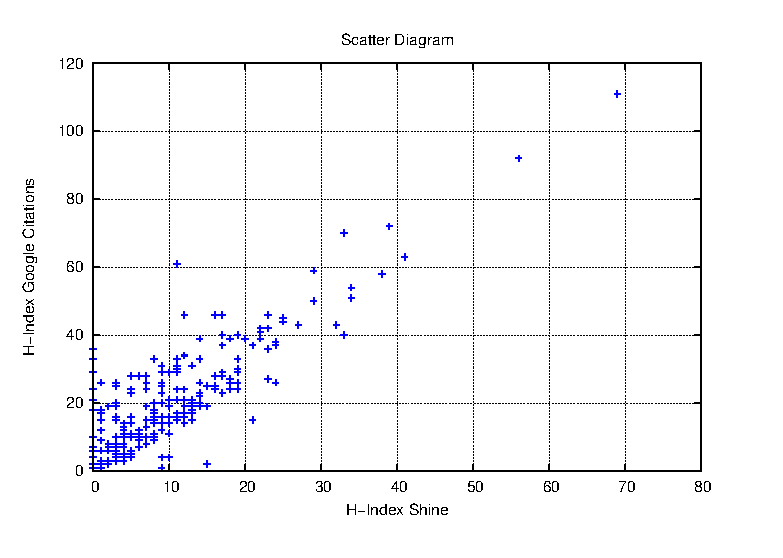
\includegraphics[scale=.5]{graficos/hindex/hindex_scatter_plot.eps}
\caption{Correlation between the inferred h-index and Google Citations one}
\vspace{-0.2cm}
\label{fig:hindex_scatter_plot}
\vspace{-0.2cm}
\end{figure}

However, there is one important limitation with this strategy.  As SHINE does not track all existing Computer Science conferences, researchers' h-index might be underestimated when computed
with this data. To investigate this issue, we compared the h-index of a set of researchers with a profile on Google Scholar with their estimated h-index based on the SHINE data. For this, we
randomly selected 10 researchers for each conference from Table~\ref{tab:sigs_conference_period} and extracted their h-indexes from their Google Scholar profiles.  In comparison
with the h-index we estimated from SHINE, the Google Scholar values are, on average, 50\% higher. Figure~\ref{fig:hindex_scatter_plot} shows the scatter plot for the two h-index
measures. We can note that although SHINE h-index is smaller, the two measures are highly correlated. The Pearson's correlation coefficient is 0.85, which indicates that researchers
might have proportional h-index estimations in both systems. 

\red{Just quickly explain the thresholds here}
Our strategy to define the two required thresholds consists of varying each of them and quantifying how they impact on the changes on the members of the community core. To measure these
changes, we compute the resemblance metric, as used in~\cite{Viswanath:2009}, which measures the fraction of members in the core at time $t_0$ that remains in the core at time $t_1$. 
For each community, we varied the window size from 1 to 5 years and the size of the community core from 10\% to 60\% of the entire community.

Intuitively, high resemblance variations indicate bad threshold choices and, thus, we should seek for values in which threshold changes cause slight changes on resemblance.
Figure~\ref{fig:averange_values_resemblance} shows the resemblance values as a function of the window size, providing different curves for the community core size.  We chose the
SIGMOD and CHI communities for this analysis. The rest of the communities are omitted due to lack of space, but the same observations hold for them. By visual inspection we would set the core
size as 10\% due to the proximity of the curves, and the window size as 2 or 3, as most of the communities showed a more stable resemblance after these values. To help us decide, we
computed the angular coefficient for the 10\% core size curves of each community and obtained the average angular coefficient for them.  Based on this value, we chose the window
size for our experiments as 3 years.


\red{Colocar um paragrafo falando da validacao}


\section{SIG Communities Structures}

\red{Put the graphs here and explain all of them.}





\section{Conclusions}





\section{Acknowledgments}

This work was partially funded by InWeb - The Brazilian National Institute
of Science and Technology for the Web (grant MCT/CNPq 573871/2008-6), and
by the authors' individual grants from CNPq, CAPES e FAPEMIG.

\bibliography{references}  % sigproc.bib is the name of the Bibliography in this case

\end{document}
